\documentclass[../main.tex]{subfiles}
\graphicspath{{\subfix{images/}}}

\begin{document}
	\section{Subsumption Test Implementation}
	As we explained before, the key part for the speed up of the algorithm it's in the subsume phase, as one of this tests is in $O(n!)$. In \cite{sortingnineinputs} they make use of Prolog's backtracking mechanism for this matter. However, this mechanism is not available in C\# (which is the programming language used for the implementation of this thesis), so I explored 2 different algorithms for skipping this permutations. Both of them make use of Lemma \ref{skipPermuationsLemma} and the $W^x$ matrices. 
	
	The first one uses a backtracking algorithm that avoids expanding branches that cannot lead to a feasible solution, and it is the one used in this thesis. The second one is extracted from \cite{improvedSubsumption} and represents the positions matrix as a bipartite graph to find possible permutations.
	
	\subsection{Permutations with backtracking}
	As an example we have the next two comparator networks represented by their comparator pairs $C_1 = [(2,4), (2,3), (1,3)]$ and $C_2=[(1,4), (3,4), (1,3)]$. Now we represent the outputs of these networks partitioned by their number of 1s (we discard the trivial outputs with all ones and all zeroes).
	
	With the partitioned sets in Table \ref{table:permutationsExample} we can create their $W^x$ matrices. Which allow us to know in which positions the outputs contain a 0 or a 1.
	
	\begin{center}
		\begin{table}[h]
			\begin{tabularx}{\textwidth}{ |l| *{3}{Y|} }
				\hline
				\textbf{number of 1s or 0s} & \textbf{1} & \textbf{2} & \textbf{3} \\
				\hline
				$W1^0$ & \makecell{1111} & \makecell{1111} & \makecell{1001} \\ [1ex]
				\hline
				$W1^1$ & \makecell{1110} & \makecell{1110} & \makecell{1111} \\  [1ex] 
				\hline
				$W2^0$ & \makecell{1111} & \makecell{1111} & \makecell{1011} \\ [1ex]
				\hline
				$W2^1$ & \makecell{1110} & \makecell{1111} & \makecell{1111} \\  [1ex] 
			\end{tabularx}
			\caption{W matrices partitioned by number of 1s or 0s}
			\label{table:whereMatrices}
		\end{table}
	\end{center}
	
	The above matrices show the positions that $x \in \{0, 1\}$ appears in the Outputs array of the comparator network. If there is a 0 in certain position it means that $x$ doesn't appear in that position in the outputs array. For example, if we look at the partition with 3 zeroes in the $W1^0$ matrix we see that 0 only appears in the positions 1 and 4.
	
	Combining the information of these 4 matrices we can obtain another matrix that will tell us the forbidden positions for the permutations. We call this matrix $P$, each row refers to an index $0,..n$ in the outputs, if there is a 0 in a specific position it means that the permutation cannot contain that number in that specific position. To create the positions matrix we iterate over the elements in $W^x$ matrices for $C_1$. If there is a 1 in that position for any of the matrices we check if there is also a 1 in the correspondent matrices of $C_2$, in that case that position is allowed and we set it to 1. For the given comparator networks we obtain the following positions matrix.
	
	\begin{figure}[H]
		$$
		\begin{bmatrix} 
			0 & 1 & 0 & 0 \\
			0 & 1 & 0 & 1 \\
			1 & 1 & 0 & 0 \\
			0 & 1 & 0 & 0 \\
		\end{bmatrix}
		\quad
		$$
		\caption{Positions matrix}
		\label{positionsMatrix}
	\end{figure}

	
	If we look carefully into the matrix, we can see that the 3rd column contains only zeroes. So, no index is allowed in the third position. This way we can say that $C_1$ does not subsume $C_2$ without trying any of the permutations. This applies also to the case that a row is all zeroes, which means that the bit in that position cannot be permuted to any of the other positions. This matrix allows to speed up the subsume operation and implement it as a backtracking algorithm which skips a huge amount of permutations. In Table \ref{table:compareSubsume} there is a comparison between the number of permutations checked while using the positions matrix with respect to not using it for comparator networks with 6 inputs.
	
	\begin{table}[H]
		\hspace*{-1.5cm}
		\begin{tabular}{|c |c c c c c c c c c c c c|}
			\hline
 			comparator & 1 & 2 & 3 & 4 & 5 & 6 & 7 & 8 & 9 & 10 & 11 & 12 \\
			\hline
			skipping & 14 & 31 & 181 & 330 & 1031 & 1373 & 1301 & 966 & 281 & 93 & 17 & 4 \\ [1ex]
			\hline
			not skipping $P$ & $2.8e3$ & $4.3e3$ & $4.5e3$ & $99e3$ & $27e4$ & $54e4$ & $59e4$ & $41e4$ & $19e4$ & $9.5e3$ & 259 & 4 \\  [1ex] 
			\hline
		\end{tabular}
		\caption{Permutations tested for $n=6$ with and without skipping permutations}
		\label{table:compareSubsume}
	\end{table}
	
	\newpage
	The Subsumes algorithm can be implemented as follows:
	
	\begin{algorithm}[H]
		\caption {Subsumes}
		\begin{algorithmic}
			\State $n$ networks input size
			\State $C_1$ comparator network
			\State $C_2$ comparator network
			\State $P$ positions matrix
			\State $j \leftarrow 0$
			\State $\pi \leftarrow \emptyset $ \Comment {permutation}
			
			\Procedure{TryPermutations}{$\pi,j$}
			\For{$i \leftarrow 1..n$}
			\If {$P[i][j] = 1$}
			\State $\pi[column] \leftarrow row $
			\If{$\textsc{TryPermutations}(\pi, column+1)$}
			\Return TRUE
			\EndIf
			\EndIf
			\EndFor
			\If {$\pi(outputs(C_2)) \subset outputs(C_1)$}
			\Return TRUE
			\Else {}
			\Return FALSE
			\EndIf
			\EndProcedure
		\end{algorithmic}
	\end{algorithm}

	\subsection{Bigraph perfect matchings}
	This approach takes into consideration the same positions matrix but, instead of the backtracking mechanism, it understand it as an adjacency matrix of a bipartite graph. A bipartite graph is composed by two disjoint sets given $G=(U,V,E)$ all edges connect $U$ with $V$. We can easily understand this as the positions where a certain bit it's allowed to be positioned.
	
	The authors of \cite{improvedSubsumption} propose an algorithm that finds all the possible permutations. For that they find all the perfect matchings in the bipartite graph. 
	
	A matching $M$ in the graph $G$ is an independent set of edges (no vertex is repeated), if that matching is of size $n$ (contains all the vertex in $U$ and $V$) we call it perfect matching. In Figure \ref{bipartite} we can find the bipartite graph representation of Figure \ref{positionsMatrix}.
	
	\begin{figure}[H]
		\begin{center}
			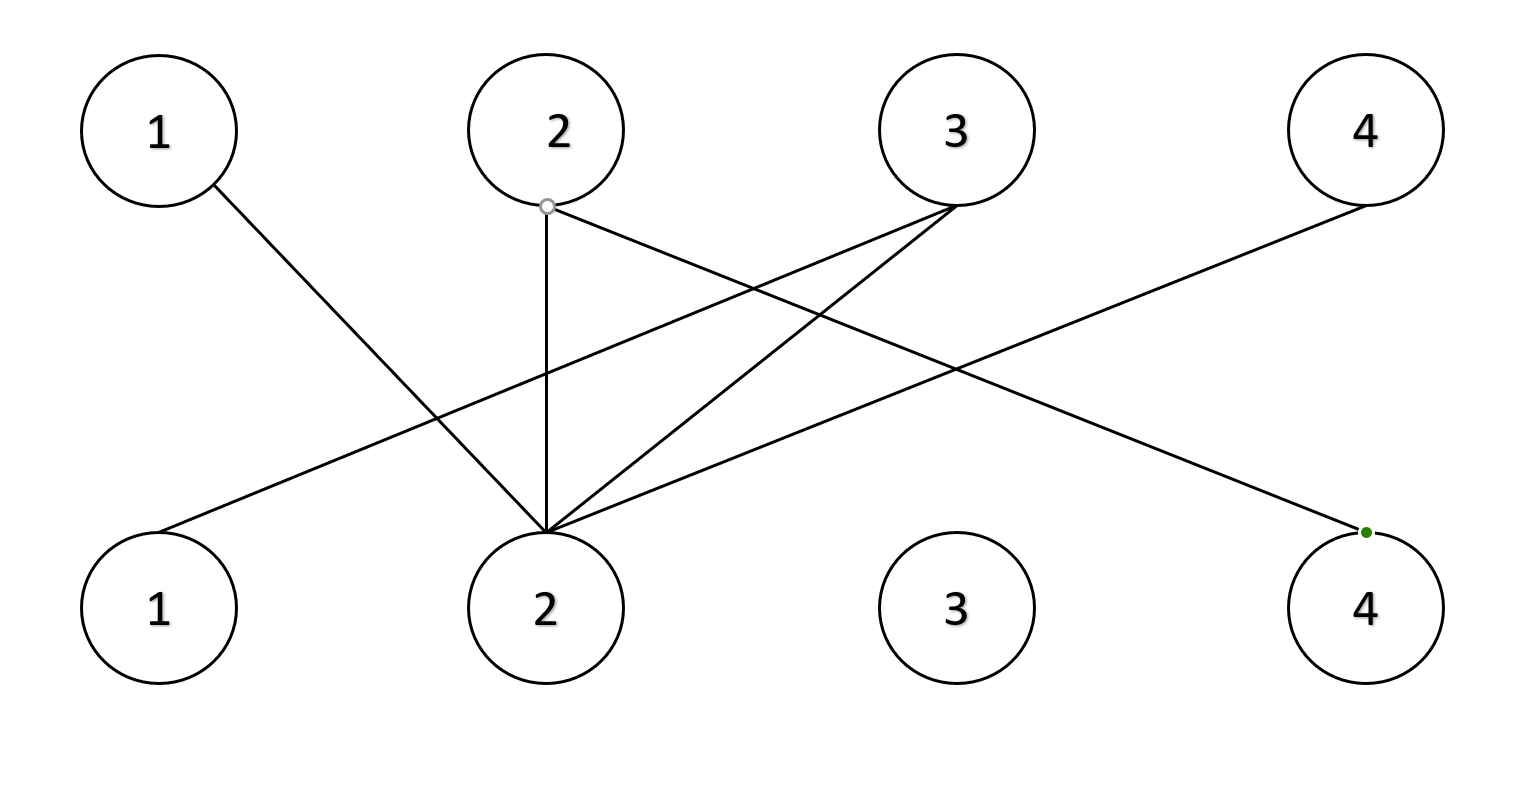
\includegraphics[width=0.7\textwidth]{images/bipartiteMatchings}
			\caption{Bipartite graph representation of the positions matrix for $C_1$ and $C_2$}
			\label{bipartite}
		\end{center}
	\end{figure}

	The authors of \cite{improvedSubsumption} introduce the following Lemma: 
	
	\begin{lemma}
		Given 2 comparator networks $C_a$ and $C_b$ with $n$ channels. If $C_a$ subsumes $C_b$ via the permutations $\pi$ then $\pi$ represents a perfect match in the bipartite graph.
	\end{lemma}

	Therefore, only the permutations that are a perfect match in the bipartite graph should be tried. 
	
	In order to obtain all the perfect matchings in the bipartite graph, they implement the algorithm in \cite{enumeratePerfectMatchings} that takes as start point a perfect matching that can be found with the Ford-Fulkerson algorithm and later finds the rest perfect matchings taking $O(n)$ time per matching.
	
	During the implementation of the thesis, I played with the idea of using this method. However, the permutations with backtracking gave better results and the results given in \cite{improvedSubsumption} state that their implementation takes more than one day of computation time in 32-core computer so we decided to not continue with this implementation.
	\newpage
\end{document}